%%%%%%%%%%%%%%%%%%%%%%%%%%%%%%%%%%%%%%%%%%%%%%%%%%%%%%%%%%%%%%%%%%%%%
%   	  UNIVERSIDADE ESTADUAL DE SANTA CRUZ-UESC                  %
%                                                                   %
%    MESTRADO EM MODELAGEM COMPUTACIONAL EM CIÊNCIA E TECNOLOGIA    %
%                                                                   %
%                    MODELO DE  DISSERTAÇÃO/TESE                    %
%                                                                   %
%                     By   Valdex Santos 							%		           
%                         <waldexsantos@gmail.com>					%
%                  		  <valdexsantos@ifba.edu.br>				%
%                         <waldexifba.wordpress.com>                %
%%%%%%%%%%%%%%%%%%%%%%%%%%%%%%%%%%%%%%%%%%%%%%%%%%%%%%%%%%%%%%%%%%%%%
%=====================================================================
\documentclass[oneside]{pacotes/ppgmc-uesc} 	% imprimir apenas frente
%\documentclass[doubleside]{pacotes/ppgmc-uesc}	% imprimir frente e verso

% importações de pacotes
	\usepackage[alf, abnt-emphasize=bf, bibjustif, recuo=0cm, abnt-etal-cite=2, abnt-etal-list=0]{abntex2cite}	% citações padrão ABNT
	\usepackage{bookmark}					% cria menu de bookmarks
	\usepackage[utf8]{inputenc}				% acentuação direta
	\usepackage[T1]{fontenc}				% codificação da fonte em 8 bits
	\usepackage{graphicx}					% inserir figuras
	\usepackage{float}				    	%PERMITE usar H em figura
	%\usepackage{picinpar}					% imagens ao lado do texto
	\usepackage{amsfonts, amssymb, amsmath}		% fonte e simbolos matemáticos
	\usepackage{cancel}                     %cancelar termos numa expressão matemática
	\usepackage{lastpage}			% Usado pela Ficha catalográfica
	\usepackage{verbatim}					% texto é interpretado como escrito no documento
	\usepackage{multirow, array}				% múltiplas linhas e colunas em     tabelas
	\usepackage{indentfirst}				% indenta o primeiro parágrafo de cada seção.
	\usepackage[algoruled, portuguese]{algorithm2e}		% escrever algoritmos

	%\usepackage{times}				    	% usa a fonte Times
	\usepackage{hyperref} 		            % inserindo links azuis, referências em preto
	\usepackage{pacotes/subfigureppgmc}					% posicionamento de figuras
	\usepackage{multicol}                   % para usar o ambiente multicols-multiplas colunas
%	\usepackage{paralist}                  %permite listas especiais
	\usepackage{xcolor, colortbl}			% comandos de cores
	%\usepackage{breakurl}					% permite quebra de linha em urls
	
	%\usepackage{subeqnarray}				% sub enumeração de equações
	%\usepackage{makeidx}					% produzir índice remissivo (glossario)
	%\usepackage{multind}					% produzir índices múltiplos
	\usepackage{pdfpages}               % inserir arq. pdf no texto (ex.: folha de aprovação e ficha catalográfica)
	\usepackage{pdflscape}                % permite colocar página em formato paisagem
%	\usepackage[normalem]{ulem} % para o underline colorido

\makeatother
 %Carrega o pacote principal
% define as cores dos links e informações do pdf
\makeatletter
\hypersetup{
	portuguese,
	colorlinks,
	linkcolor=blue,
	citecolor=blue,
	filecolor=blue,
	urlcolor=blue,
	breaklinks=true,
	pdftitle={\@title},
	pdfauthor={\@author},
	pdfsubject={\imprimirpreambulo},
	pdfkeywords={abnt, latex, abntex, abntex2}
} %carrega as configurações de cores
% inclui informações sobre AUTORIA, INSTITUIÇÃO e ORIENTAÇÃO do trabalho
%======================================================================================================
%DADOS DO TRABALHO
%****************************************************************************************************
\titulo{Template \LaTeX \ para  Trabalho de conclusão  de Curso de  Mestrado ou Doutorado\par PPGMC -- UESC}
\titleenglish{LaTeX Class for Graduation Course (monograph), Master's or Doctorate work\par PPGMC - UESC }
%\subtitulo{Subtítulo do trabalho}
\autor{Valdex de Jesus Santos}
\tipotrabalho{Dissertação (Mestrado)} %troque por Tese (Doutorado) para tese de doutorado ou monografia se for o caso
\preambulo{Dissertação apresentada ao Programa de Pós-Graduação em Modelagem Computacional em Ciência e Tecnologia da  Universidade Estadual de Santa Cruz, como parte das exigências para obtenção do título de Mestre  em Modelagem Computacional em Ciência e Tecnologia.}
%========================================================================================================
%======================================================================================================
%ORIENTAÇÃO DO TRABALHO
%****************************************************************************************************
\orientador{Prof. Dr. Fulano de tal}  %Para orientadora:\orientador[Orientadora:]{Nome da orientadora}
\coorientador{Prof. Dr. Ciclano de tal} %para coorientadora: \coorientador[Coorientadora:]{Nome da coorientadora}
\instCoorientador{UESC} %Necessário, pois o Coorientador pode ser de outra instituição
%\areaconcentracao{Modelagem Matemática e Computacional} %Não necessário no modelo 	UESC
%\linhapesquisa{Sistemas Inteligentes} %Não necessário no modelo UESC (caso necessário na sua intituição, descomente)
%========================================================================================================

%======================================================================================================
%DADOS DA INSTITUIÇÃO
%****************************************************************************************************
\local{Ilhéus-BA} %coloque o nome da cidade da sua instituição
\data{2020} %ano de defesa
\programa{Programa de Pós-Graduação em Modelagem Computacional\par em Ciência e Tecnologia}
\instituicao{%
 UNIVERSIDADE ESTADUAL DE SANTA CRUZ

\par
PRO-REITORIA DE PESQUISA E PÓS-GRADUAÇÃO
}
%========================================================================================================

%======================================================================================================
%DADOS DA DEFESA
%****************************************************************************************************
%caso você não tenha coorienador comente a linha 38 do arquivo folhaAprovacao na pasta 01-Elementos-pre-textuais
\datadefesa{23/06/2020} %Coloque  data de defesa

\bancamembrointerno{Prof. Dr. Membro Interno} %Coloque o nome do membro interno que fará parte da banca
\bancainstmembrointerno{UESC} %Coloque o nome ou sigla da instituição do membro interno que fará parte da banca

\bancamembroexterno{Prof. Dr. Membro Externo} %Coloque o nome do membro externo que fará parte da banca
\bancainstmembroexterno{UERJ} %Coloque o nome ou sigla da instituição do membro externo que fará parte da banca


%========================================================================

% INICIO DO DOCUMENTO
\begin{document}
\pretextual
% retira espaço extra obsoleto entre as frases.
\frenchspacing

% elementos pré textuais
		
	\imprimircapa						% Capa- elemento obrigatório 
	\imprimirfolhaderosto{}					% Folha de rosto-- elemento obrigatório
%	% FICHA CATALOGRÁFICA

\includepdf[pages=1]{FichaCatalografica.pdf}	% Ficha catalográfica-- elemento obrigatório
	%
% Documento: Folha de aprovação
%
\makeatletter
\begin{folhadeaprovacao}

	\begin{center}
		{\large\normalfont\scshape\textbf\imprimirautor}
	\end{center}

	\vspace*{50pt}

	\begin{center}
		\ABNTEXchapterfont\Large\scshape\imprimirtitulo
		\abntex@ifnotempty{\imprimirsubtitulo}{
			{\ABNTEXchapterfont\Large\scshape{\hspace*{-0.3em}: }}{\ABNTEXchapterfont\large\scshape\imprimirsubtitulo}
		}
	\end{center}

	\vspace*{30pt}

%	\abntex@ifnotempty{\imprimirpreambulo}{
%		\SingleSpacing
%		\begin{tabular}{p{.25\textwidth}p{.13\textwidth}p{.44\textwidth}}
%			& \multicolumn{2}{p{.6\textwidth}}{\small\hyphenpenalty=10000{\imprimirpreambulo}} \\ & & \\
%		\end{tabular}
%	}
%
%	\vspace*{7pt}

	\begin{center}
		\imprimirlocal, \imprimirdatadefesa
		\end{center}
		
		\vspace*{7pt}
		\begin{center}
		Comissão Examinadora
		\end{center}
\vspace{-2pt}
\begin{center}
\begin{tabular}{cc}
	\assinatura{\textbf{\imprimirorientador} \\ UESC\\ (Orientador)}&\\
		\assinatura{\textbf{\imprimircoorientador} \\ \imprimirinstCoorientador\\ (Coorientador)}&\\ 
		\assinatura{\textbf{\imprimirbancamembrointerno} \\ \imprimirbancainstmembrointerno} &\\
		\assinatura{\textbf{\imprimirbancamembroexterno} \\ \imprimirbancainstmembroexterno}&\\
	
\end{tabular}
	
	\end{center}
%	\begin{center}
%		\assinatura{\textbf{\imprimirorientador} \\ Orientador} 
%		\assinatura{\textbf{Professor} \\ Convidado 1}
%		\assinatura{\textbf{Professor} \\ Convidado 2}
%		%\assinatura{\textbf{Professor} \\ Convidado 3}
%		%\assinatura{\textbf{Professor} \\ Convidado 4}
%	\end{center}

%	\vspace*{\fill}

%	\begin{center}
%		\normalfont\scshape{\imprimirinstituicao}\\
%		\normalfont\scshape{\imprimirprograma}\\
%		\normalfont\scshape{\imprimirlocal}\\
%		\normalfont\scshape{\imprimirdata}
%	\end{center}

\end{folhadeaprovacao}
%\makeatother
	% Folha de aprovação-- elemento obrigatório
	%
% Documento: Dedicatória
%

\begin{dedicatoria}

Espaço reservado para dedicatória.
Inserir seu texto aqui...

\end{dedicatoria}
	% Dedicatória-- elemento opcional, comente se não for colocar
	%
% Documento: Agradecimentos
\pagestyle{empty}

\begin{agradecimentos}
\begin{incisos}
\item Nesta parte o discente pode agradecer a quem quiser.
\item A ordem em que aparecem aqueles a quem se agradece pressupõem a ordem de importância para que o seu trabalho fosse realizado: quem lhe ofereceu a oportunidade de trabalho, quem financiou o seu trabalho, quem efetivamente contribuiu cientificamente durante a discussão do seu trabalho, quem efetivamente resolveu problemas da parte experimental do seu trabalho.
\item Os seus colegas de trabalho que contribuíram para a boa convivência no seu local de trabalho
\item Os técnicos, secretários, e afins que contribuíram para a realização do seu trabalho
\item 	A sua família e membros presentes ou ausentes que merecem ser lembrados mas que não contribuíram fisicamente para a realização do seu trabalho no local de trabalho.
\item Não se deve preferencialmente confundir aspectos religiosos com acadêmicos. O trabalho de conclusão é o resultado de hipótese, experimentação, resultados e discussão científica. 
\end{incisos}

\end{agradecimentos}
% Agradecimentos-- elemento opcional, comente se não for colocar
	%
% Documento: Epígrafe
%

\begin{epigrafe}

\textit{``Aqui fica o seu epígrafe.''}

\end{epigrafe}
		% Epígrafe-- elemento opcional, comente se não for colocar
	%
% Documento: Resumo (Português)
%


\begin{center}
\imprimirtitulo
\end{center}

\begin{resumo}
Síntese do trabalho em texto cursivo contendo um único parágrafo. O resumo é a apresentação clara, concisa e seletiva do trabalho.
No resumo deve-se incluir, preferencialmente, nesta ordem: brevíssima introdução ao assunto do trabalho de pesquisa (qualificando-o quanto à sua natureza), o que será feito no trabalho (objetivos), como ele será desenvolvido (metodologia), quais serão os principais resultados e conclusões esperadas, bem como qual será o seu valor no contexto acadêmico. Para o projeto de dissertação e teses sugere-se que o resumo contenha de 150 a 500 palavras, de acordo com as normas da UESC \cite{normasuesc}. Caso esteja utilizando este modelo em outra instituição, observe as normas da mesma para o resumo.

\textbf{Palavras-chave}: latex. abntex. modelo.
 \textit{(Entre 3 a 6 palavras ou termos, separados por ponto, descritores do trabalho. As palavras-chaves são Utilizadas para indexação).}

\end{resumo}
		% Resumo na língua vernácula-- elemento obrigatório
	%
% Documento: Resumo (Inglês)
%


\begin{center}
\imprimirtitleenglish
\end{center}

\begin{resumo}[Abstract]
	Translation of the abstract into english, possibly adapting or slightly changing the text in order to adjust it to the grammar of english educated.

	\textbf{Keywords}: latex. abntex. template.

\end{resumo}
		% Resumo em língua estrangeira-- elemento obrigatório
	%
% Documento: Lista de figuras
%

\pdfbookmark[0]{\listfigurename}{lof}
\listoffigures*
\cleardoublepage
	% Lista de figuras-- elemento obrigatório caso tenha figuras no seu texto
	%
% Documento: Lista de tabelas
%

\pdfbookmark[0]{\listtablename}{lot}
\listoftables*
\cleardoublepage
	% Lista de tabelas-- elemento obrigatório caso tenha tabelas no seu texto
	%
% Documento: Lista de quadros
%

\pdfbookmark[0]{\listofquadrosname}{loq}
\listofquadros*
\cleardoublepage
	% Lista de quadros-- elemento obrigatório caso tenha quadros no seu texto
%%	%
% Documento: Lista de algoritmos
%

\newcommand{\algoritmoname}{Algoritmo}
\renewcommand{\listalgorithmcfname}{Lista de algoritmos}

\floatname{algocf}{\algoritmoname}
\newlistof{listofalgoritmos}{loa}{\listalgoritmoname}
\newlistentry{algocf}{loa}{0}

\counterwithout{algocf}{chapter}
\renewcommand{\cftalgocfname}{\algoritmoname\space}
\renewcommand*{\cftalgocfaftersnum}{\hfill--\hfill}

\pdfbookmark[0]{\listalgorithmcfname}{loa}
\listofalgorithms
\cleardoublepage
	% Lista de algoritmos caso tenha algoritmos
	%
% Documento: Lista de abreviaturas e siglas
%

\begin{siglas}
	\item[UESC] Universidade Estadual de Santa Cruz
	\item[DCET] Departamento de Ciências Exatas e Tecnológicas
	\item[PPGMC] Programa de Pós-Graduação em Modelagem Computacional em Ciência e Tecnologia
\end{siglas}
	% Lista de abreviaturas e siglas caso tenha usado no texto
	%
% Documento: Lista de símbolos
%

\begin{simbolos}
	\item[$ \Gamma $] Letra grega Gama
	\item[$ \lambda $] Comprimento de onda
	\item[$ \in $] Pertence
\end{simbolos}
	% Lista de símbolos-- elemento opcional
	%
% Documento: Sumário
%

\pdfbookmark[0]{\contentsname}{toc}
\tableofcontents*
\cleardoublepage		% Sumário-- elemento obrigatório
%=======================================================================================================================
% elementos textuais
	\textual

	%
% Documento: Introdução
%

\chapter{Introdução}\label{chap:introducao}
Este template em \LaTeX \ de trabalho de final de curso foi elaborado para o programa de Pós-Graduação em Modelagem Computacional em Ciência e Tecnologia, mas também pode ser utilizado por outros programas de graduação e pós-graduação da UESC e até de outras instituições, caso se adéque as regras da mesma.

Para tanto, elaboramos a classe {\ttfamily ppgmc-uesc.cls}, construída com base nas normas da ABNT e da UESC para trabalhos de conclusão de curso. Maiores detalhes relacionados aos comandos existentes no estilo podrão da ABNT devem ser adquiridos através da documentação disponível no site \href{http://www.abntex.net.br/}{http://www.abntex.net.br/}. Encorajamos a consultar as regras do pacote abntex  \href{http://linorg.usp.br/CTAN/macros/latex/contrib/abntex2/doc/abntex2.pdf}{neste link}.

Para melhor entendimento do uso do estilo de formatação, aconselha-se que o  usuário analise os comandos existentes no arquivo {\ttfamily PPGMC.tex} e os resultados obtidos após copilação.

Os arquivos pré-textuais, textuais e pós-textuais podem ser modificados a vontade. Nas pastas contém apenas exemplos. As referências citadas também são apenas exemplos, não se referindo necessariamente as informações anunciadas. O arquivo principal {\ttfamily PPGMC.tex} também pode ser modificado ou renomeado.

A utilização desse template requer conhecimento prévio de Latex. A primeira versão foi lançada em 2015 para uso em editores offline. Agora estamos lançado este template online na plataforma \href{https://pt.overleaf.com}{\ttfamily \textit{overleaf}}. Sugestões de como melhorá-la e indicação de possíveis correções serão muito bem recebidas. A partir do segundo capítulo descrevemos como utilizar este template. Na seção \ref{sec:contatos} estão os contatos do autor para dúvidas e contribuições.

\section{Motivação}
\label{sec:motivacao}

Tendo em vista que o programa de Pós-Graduação em Modelagem Computacional em Ciência e Tecnologia ainda não tinha um estilo padrão para teses e dissertações, nem mesmo a UESC, resolveu desenvolver um template de padronização dos trabalhos do programa e demais programas de mestrado e doutorado da UESC. Um modelo de TCC da UESC pode ser encontrado \href{https://www.overleaf.com/latex/templates/modelo-tcc-uesc/sqtswzxtgwkj}{neste link}. Nada impede que este modelo seja utilizado também por programas de outras universidades, caso as regras sejam as mesmas ou possam ser modificadas nos arquivos aqui contidos.

O estilo de documento utilizado é o {\ttfamily abntex2}. Através desse estilo a constituição do documento torna-se facilitada, uma vez que o mesmo possui comandos especiais para auxiliar a distribuição/definição das diversas partes constituintes do projeto. 


Uma das principais vantagens do uso do estilo de formatação para LATEX é a formatação \textit{automática} dos elementos que compõem um documento acadêmico, tais como capa, folha de rosto, dedicatória, agradecimentos, epígrafe, resumo, abstract, listas de figuras, tabelas, siglas e símbolos, sumário, capítulos, referências etc.


		%introdução
	
\chapter{Chamada dos arquivos dentro do código principal}
O arquivo principal a ser copilado é {\ttfamily PPGMC.tex}. Nele são chamados os  arquivos/elementos da sua dissertação (ou tese). Faça as modificações após o comando \verb#\begin{document}#. Depois abra cada um dos documentos que estão sendo chamados pelo documento mestre e modifique-os para obter o seu documento final. Todos os arquivos dos elementos pré-textuais, textuais e pós-textuais devem ser editados pelos autores, segundo suas necessidades.

\section{Arquivos, Pacotes e configurações}
O arquivo {\ttfamily pacoteprincipal.tex}, chamado no arquivo principal com o comando \verb#\documentclass[oneside]{pacotes/ppgmc-uesc} 	% imprimir apenas frente
%\documentclass[doubleside]{pacotes/ppgmc-uesc}	% imprimir frente e verso

% importações de pacotes
	\usepackage[alf, abnt-emphasize=bf, bibjustif, recuo=0cm, abnt-etal-cite=2, abnt-etal-list=0]{abntex2cite}	% citações padrão ABNT
	\usepackage{bookmark}					% cria menu de bookmarks
	\usepackage[utf8]{inputenc}				% acentuação direta
	\usepackage[T1]{fontenc}				% codificação da fonte em 8 bits
	\usepackage{graphicx}					% inserir figuras
	\usepackage{float}				    	%PERMITE usar H em figura
	%\usepackage{picinpar}					% imagens ao lado do texto
	\usepackage{amsfonts, amssymb, amsmath}		% fonte e simbolos matemáticos
	\usepackage{cancel}                     %cancelar termos numa expressão matemática
	\usepackage{lastpage}			% Usado pela Ficha catalográfica
	\usepackage{verbatim}					% texto é interpretado como escrito no documento
	\usepackage{multirow, array}				% múltiplas linhas e colunas em     tabelas
	\usepackage{indentfirst}				% indenta o primeiro parágrafo de cada seção.
	\usepackage[algoruled, portuguese]{algorithm2e}		% escrever algoritmos

	%\usepackage{times}				    	% usa a fonte Times
	\usepackage{hyperref} 		            % inserindo links azuis, referências em preto
	\usepackage{pacotes/subfigureppgmc}					% posicionamento de figuras
	\usepackage{multicol}                   % para usar o ambiente multicols-multiplas colunas
%	\usepackage{paralist}                  %permite listas especiais
	\usepackage{xcolor, colortbl}			% comandos de cores
	%\usepackage{breakurl}					% permite quebra de linha em urls
	
	%\usepackage{subeqnarray}				% sub enumeração de equações
	%\usepackage{makeidx}					% produzir índice remissivo (glossario)
	%\usepackage{multind}					% produzir índices múltiplos
	\usepackage{pdfpages}               % inserir arq. pdf no texto (ex.: folha de aprovação e ficha catalográfica)
	\usepackage{pdflscape}                % permite colocar página em formato paisagem
%	\usepackage[normalem]{ulem} % para o underline colorido

\makeatother
#, contém os principais pacotes utilizados. Já o comando \verb#% define as cores dos links e informações do pdf
\makeatletter
\hypersetup{
	portuguese,
	colorlinks,
	linkcolor=blue,
	citecolor=blue,
	filecolor=blue,
	urlcolor=blue,
	breaklinks=true,
	pdftitle={\@title},
	pdfauthor={\@author},
	pdfsubject={\imprimirpreambulo},
	pdfkeywords={abnt, latex, abntex, abntex2}
}}# chama o arquivo de configurações de cores. Ambos os arquivos estão na  {\ttfamily pasta pacotes}. Ainda nesta mesma pasta está pacote \verb#subfigureppgmc# necessário para colocar figura lado a lado, conforme explicado na subseção \ref{figladoalado} e o arquivo {\ttfamily ppgmc-uesc} que contém toda a programação da classe. Esses arquivos não devem ser apagados ou alterados.

o comando \verb#\pretextual# indica o início da chamada dos elementos obrigatórios e opcionais. Os comandos  \verb#\imprimircapa# e \verb#\imprimirfolhaderosto{}# imprimem a capa e  a folha de rosto, respectivamente, com as informações contida no arquivo {\ttfamily 1-Inf.Capa-FolhaRosto} na pasta {\ttfamily 01-elementos-pre-textuais}. Tanto a capa quanto a folha de rosto são obrigatórias segundo as normas da ABNT e da UESC.

\textit{No arquivo \textit{{\ttfamily 1-Inf.Capa-FolhaRosto}} referido é que você dever colocar as informações principais do seu trabalho, tais como: título, autor, orientador, coorientador (caso não tenha coorientador comente a linha), instituição, tipo de trabalho (dissertação ou tese) etc. Tais informações aparecerão automaticamente na capa, folha de rosto, folha de aprovação.}

Este template leva em consideração que o autor possui coorientador, caso não possua basta comentar a linha 43 do arquivo \textit{{\ttfamily FolhaAprovacao}}, também na pasta {\ttfamily 01-elementos-pre-textuais}.


Na pasta {\ttfamily 01-elementos-pre-textuais} estão exemplos de arquivos pré-textuais, chamados no arquivo principal, a saber:
\begin{alineas}
\item \textbf{FolhaAprovacao}  -- elemento obrigatório
\item \textbf{dedicatoria} -- elemento opcional
\item \textbf{agradecimentos} -- elemento opcional
\item \textbf{epigrafe} -- elemento opcional
\item \textbf{resumoPt} -- elemento obrigatório
\item \textbf{resumoEn} -- elemento obrigatório
\item \textbf{listaFiguras} -- elemento opcional
\item \textbf{listaTabelas} -- elemento opcional 
\item \textbf{listaQuadros} -- elemento opcional 
\item \textbf{listaAlgoritmos} -- elemento opcional
\item \textbf{listaSiglas} -- elemento opcional
\item \textbf{listaSimbolos} -- elemento opcional
\item \textbf{sumário} -- elemento obrigatório
\end{alineas}

Os arquivos {\ttfamily listaFiguras, listaTabelas, listaQuadros e listaAlgoritmos} não precisam ser modificados. Caso algum destes elementos não seja necessário no seu trbalho, simplesmente comente no arquivo principal. Os arquivos  {\ttfamily listaSiglas e listaSimbolos} devem ser editados se fizerem parte do seu trabalho, caso contrário comente no arquivo principal.

A \textit{ficha catalográfica} é um elemento obrigatório fornecida pela biblioteca e deve ser colocado no verso da folha de rosto. No arquivo principal, a linha correspondente está comentada. Após ter em mão essa ficha, fornecida pela sua biblioteca, faça upload do arquvivo renomeado para \textit{{\ttfamily FichaCatalografica}} e descomente a linha correspondente no arquivo principal. 

O comando 	\verb#\textual# indica o início dos elementos textuais que são constituídos pela introdução, capítulos e conclusão. Já o comando \verb#\postextual# marca o início dos elementos pós-textuais, os quais são: referências, glossário, apêndices e índices. As referências devem ser armazenadas num arquivo de extensão \verb#.bib#. Na pasta \verb#03-elementos-pos-textuais# tem o arquivo {\ttfamily refbase.bib} que contém uma quantidade de referências como exemplo. Você pode substituir as que estão nesse arquivo pelas suas, sem necessidade de criar um novo arquivo. O capítulo \ref{chap:conclusao} traz mais detalhes.
\section{Coleta de dados}

Inserir seu texto aqui...

	% Elementos da dissertação/tese
	%
% 
%

\chapter{Citações e Referências}\label{referencias}
Neste capítulo, assim como nos anteriores procuramos inserir muitas citações bibliográficas a fim de familiarizar os autores com as diferentes maneiras de fazê-las, nesse sentido o template é bastante versátil. Os principais itens de bibliografia citados são livros, artigos em conferências,
artigos em jornais e páginas Web. A bibliografia deve seguir as normas da ABNT e também da UESC.

Citações são trechos transcritos ou informações retiradas das publicações consultadas para a realização do trabalho.
As citações são utilizadas no texto com o propósito de esclarecer, completar, embasar ou corroborar as ideias do autor.

Todas as publicações consultadas e efetivamente utilizadas (através de citações) devem ser listadas, obrigatoriamente, nas referências bibliográficas, de forma a preservar os direitos autorais e intelectuais, conforme consta nas normas da ABNT e da UESC.

A bibliografia é feita no padrão {\ttfamily bibtex}. As referências são colocadas em um arquivo separado. Nesse caso o arquivo  {\ttfamily refbase}. Fizemos questão de colocar uma referência de cada formato de fontes mais populares: livros, jornais, mídias na internet etc.

Os elementos de cada item bibliográfico que devem constar na bibliografia são apresentados a seguir.

Para livros, o formato da bibliografia no arquivo fonte é o seguinte:

\begin{verbatim}
@Book{linked,
   author = {A. L. Barabasi},
   title = {Linked: The New Science of Networks},
   publisher = {Perseus Publishing},
   year = {2002},
}
\end{verbatim}

A citação deste livro se faz da seguinte forma \verb#\cite{linked}# e o resultado fica assim \cite{linked}.
Para os artigos em {\textit jornais}, veja por exemplo \cite{carvalho:2001},
descrito da seguinte forma no arquivo {\ttfamily .bib}:

\begin{verbatim}
@Article{carvalho:2001,
  Title = {Inteligência competitiva numa visão de futuro},
  Author= {Cláudia Carvalho and José Fajardo and Joaquim Cruz},
  Journal = {DataGramaZero - Revista da Ciência da Informação},
  Year = {2001},
  Number= {3},
  Pages = {12--16},
  Volume = {2},

  Mounth= {junho},
  Subtitle = {proposta metodológica}
}
\end{verbatim}


\section{Citação indiretas ou livres}\label{ciação direta}

As citações indiretas são feitas com base no comando \verb|\citeonline{label}|, onde \verb|label| corresponde a um nome dado para chamar a referência no texto. O comando \verb|\citeonline{maturana:2003}| gera a seguinte citação indireta: \citeonline{maturana:2003} defende um princípio de lógica...

Além disso, \citeonline{teste:2014} argumenta que \ldots\mbox{ } Observe o detalhe do termo \textit{et al}.
que deve ser utilizado quando o trabalho citado possui mais de três autores. Este é o padrão do estilo {\ttfamily abntex2}.

Para evitar uma interrupção na sequência do texto, o que poderia, eventualmente, prejudicar a leitura, pode-se indicar a fonte entre parênteses imediatamente após a citação indireta. Porém, neste caso específico, o nome do autor deve vir em caixa alta, seguido do ano da publicação, como no exemplo a seguir.

A física, então, constituiu-se como a prova mínima da efetividade do método científico para descobrir as verdades do universo \cite{teste:2014,maturana:2003}. Essa citação foi obtida com o comando \verb|\cite{teste:2014,maturana:2003}|


\section{Citações diretas ou literais}\label{citacoesdiretas}

Há várias maneiras de se fazer uma citação literal, como mostra os exemplos abaixo.

As citações longas (mais de 3 linhas) devem usar um parágrafo específico para ela, na forma de um texto recuado (4 cm da margem esquerda), com tamanho de letra menor do aquela utilizada no texto e espaçamento simples entre as linhas, seguido dos sobrenomes dos autores em caixa alta (separados por ponto e vírgula), ano de publicação e número da página.

As citações diretas são obtidas com o comando \verb|\cite{label}|. Veja o exemplo abaixo onde usamos o ambiente citação e o comando \verb|\cite[p.~28]{morinmoigne:2000}| para citar o autor.

\begin{citacao}
Desse modo, opera-se uma ruptura decisiva entre a reflexividade filosófica, isto 	é a possibilidade do sujeito de pensar e de refletir, e a objetividade científica.
Encontramo-nos num ponto em que o conhecimento científico está sem consciência.
Sem consciência moral, sem consciência reflexiva e também subjetiva.
Cada vez mais o desenvolvimento extraordinário do conhecimento científico vai tornar menos praticável a própria possibilidade de reflexão do sujeito sobre a sua pesquisa \cite[p.~28]{morinmoigne:2000}.
\end{citacao}

A sintaxe do ambiente citação utilizado acima é a seguinte:
\begin{verbatim}
    \begin{citacao}
        <citacao>
    \end{citacao}
\end{verbatim}

Opcionalmente, pode-se referenciar os autores no corpo de texto (neste caso seus nomes devem vir em minúsculas), e em seguida colocar a citação literal, em um novo parágrafo recuado. Nesse caso após a citação literal não mais aparece o nome dos autores, visto que já se encontra no texto.
Veja o exemplo seguinte.

\citeonline[p.~33]{morinmoigne:2000}, ao fazerem as suas críticas à ciência, explicitam uma ideia coletiva:

\begin{citacao}
Mas o curioso é que o conhecimento científico que descobriu os meios realmente extraordinários para, por exemplo, ver aquilo que se passa no nosso sol, para tentar conceber a estrutura das estrelas extremamente distantes, e até mesmo para tentar pesar o universo, o que é algo de extrema utilidade, o conhecimento científico que multiplicou seus meios de observação e de concepção do universo, dos objetos, está completamente cego, se quiser considerar-se apenas a si próprio!
\end{citacao}

As citações curtas (menos de 3 linhas) devem ser inseridas diretamente no texto (entre aspas), seguida do nome do autor (em caixa alta), ano e página, como no exemplo a seguir.

Então significa apenas que ``assumo que não posso fazer referência a entidades independentes de mim para construir meu explicar'' \cite[p.~35]{maturana:2003}.

\section{Resumo dos comandos para  referências }\label{referenciasUtilizadas}

Apresentamos abaixo exemplos de referências já citadas no texto com seus comandos.

\begin{itemize}
	\item \citeonline{maturana:2003}\\ \verb|\citeonline{maturana:2003}|
	\item \citeonline{teste:2014}\\ \verb|\citeonline{teste:2014}|
	\item \cite[p.~28]{morinmoigne:2000}\\ \verb|\cite[p.~28]{morinmoigne:2000}|
	\item \citeonline[p.~33]{morinmoigne:2000}\\ \verb|\citeonline[p.~33]{morinmoigne:2000}|
	\item \cite[p.~35]{maturana:2003}\\ \verb|\cite[p.~35]{maturana:2003}|
	\item \citeonline[p.~35]{maturana:2003}\\ \verb|\citeonline[p.~35]{maturana:2003}|
	\item \cite{teste:2014,maturana:2003}\\ \verb|\cite{teste:2014,maturana:2003}|
\end{itemize}
	% citações e referências
	
\chapter{Figuras, Tabelas e outros elementos}\label{chap:fundamentacaoTeorica}
A seguir ilustra-se a forma de incluir figuras, tabelas, equações, siglas e símbolos no documento, obtendo indexação automática em suas respectivas listas.
A numeração sequencial de figuras, tabelas e equações ocorre de modo automático.
Referências cruzadas são obtidas através dos comandos \verb#\label{}# e \verb#\ref{}#.
Por exemplo, estou me referindo agora a introdução que corresponde ao  capítulo \ref{chap:introducao}. Todos os comandos utilizados para gerar os elementos desse texto estão nos respectivos arquivos dos capítulos. Não os colocaremos aqui para que o texto não fique demasiadamente extenso e não ficarmos repetitivos.

\section{Figuras}
\label{sec:figuras}

Abaixo é apresentado um exemplo de figura. A  figura \ref{fig:brasaouesc} aparece automaticamente na lista de figuras. Para uso avançado de imagens no LATEX, recomenda-se a consulta de literatura especializada.

\begin{figure}[!htb]
\centering
	
\includegraphics[width=0.3\textwidth]{./04-figuras/brasaouesc}\label{fig:brasaouesc}
    \caption{Brasão da UESC}\vspace{-0.4cm}
    \fonte{\citeonline{teste:2014}}

\end{figure}

\subsection{Figuras lado a lado}\label{figladoalado}
Para colocar figuras lado a lado com legendas diferentes utilizamos o pacote {\ttfamily subfigure}, declarado no preâmbulo. Porém o pacote abntex, no qual nos baseamos, é incompatível com o pacote {\ttfamily subfigure}. Ao tentar usá-lo a compilação apresenta erros de incompatibilidade. 

Para contornar essa situação fiz algumas alterações necessárias no pacote e o renomeei como {\ttfamily subfigureppmgc}. Assim, caso você queira utilizar no seu texto figuras lado a lado com legendas diferentes, deve utilizar essa nova versão do  pacote, o qual se encontra na pasta {\ttfamily pacotes}. O template já está configurada para utilizá-lo automaticamente.

Caso as figuras que fiquem lado a lado  utilizem apenas uma legenda não há necessidade do pacote, basta chamá-las normalmente no ambiente {\ttfamily figure}.

Abaixo segue um exemplo de como fica a utilização do pacote inserindo figuras lado a lado, com legendas diferentes.\\

\begin{figure}[!htb]
 \subfigure[\label{fig:rc-adezanoss}]{
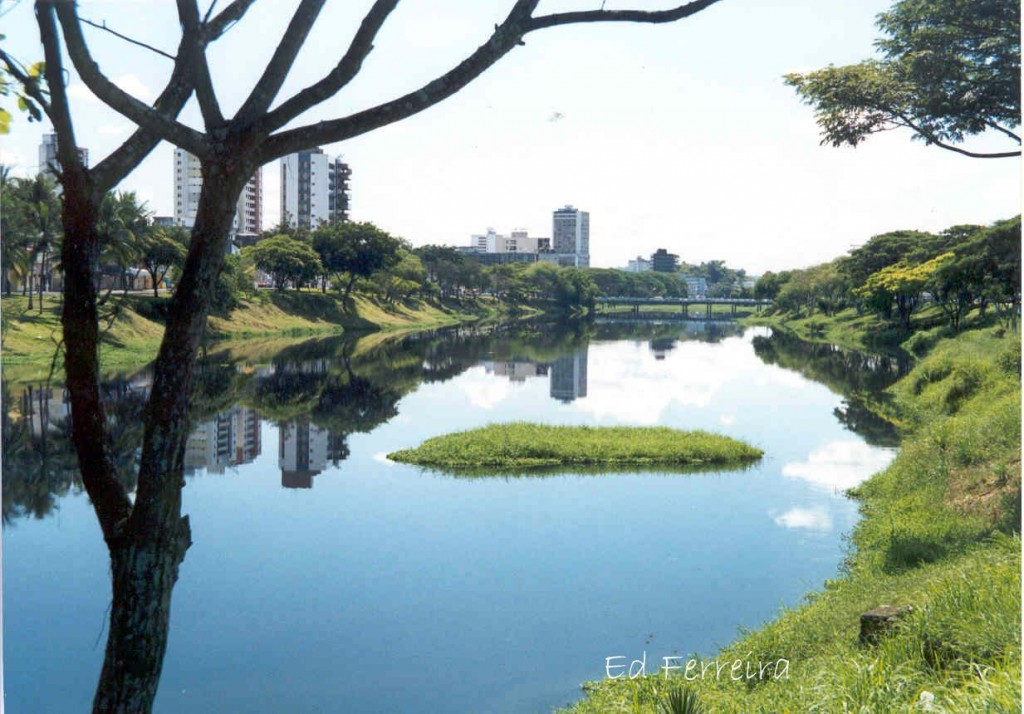
\includegraphics[width=7cm,height=6cm]{04-figuras/rc-adezanos}}
\subfigure[\label{fig:rc-atualmentee}]{
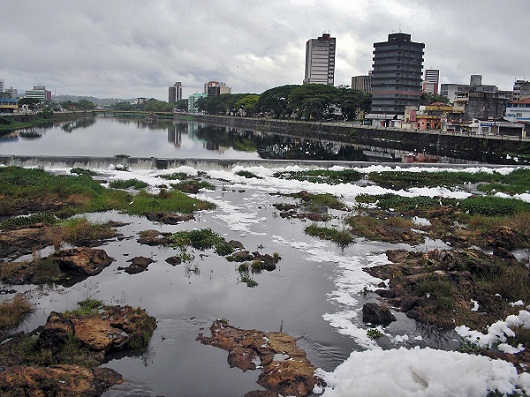
\includegraphics[width=7cm,height=6cm]{04-figuras/rc-atualmente}}
\caption{Imagens comparando  o rio Cachoeira a dez anos atrás (a)  e em 2013 (b)} \label{fig:estadorc}\vspace{-0.6cm}
\fonte{Pimenta Blog.BR, no endereço em $<$http://www.pimenta.blog.br/$>$}
\end{figure}

Este \href{https://www.overleaf.com/learn/latex/Inserting_Images}{link do overleaf} contém mais informações de como trabalhar com figuras em latex. 
\section{Quadros e Tabelas}
\label{sec:tabelas}

Também é apresentado o exemplo do quadro \ref{qua:comparabd} e da tabela \ref{tab:correlacao}, que aparece automaticamente na lista de quadros e tabelas.
Informações sobre a construção de tabelas no LATEX podem ser encontradas na literatura especializada e neste link de ajuda do overleaf: \href{https://www.overleaf.com/learn/latex/Tables}{https://www.overleaf.com/learn/latex/Tables}.

\begin{quadro}[!htb]
	\centering
	\caption{Hierarquia de restrições das questões.\label{qua:comparabd}}
	\begin{tabular}{|p{7cm}|p{7cm}|}
		\hline
		\textbf{BD Relacionais} & \textbf{BD Orientados a Objetos} \\
		\hline
		Os dados são passivos, ou seja, certas operações limitadas podem ser automaticamente acionadas quando os dados são usados. Os dados são ativos, ou seja, as solicitações fazem com que os objetos executem seus métodos. & Os processos que usam dados mudam constantemente. \\
		\hline
	\end{tabular}
	\fonte{\citeonline{teste:2014}}
\end{quadro}

\newpage
\textbf{Exemplos de tabelas:
}
\begin{table}[!htb]
	\centering
	\caption[Correlação de valores x e y]{Exemplo de uma tabela mostrando a correlação entre x e y.\label{tab:correlacao}}
	\begin{tabular}{cc}
		\hline
			x & y \\
		\hline
			1 & 2 \\
			3 & 4 \\
			5 & 6 \\
			7 & 8 \\
		\hline
	\end{tabular}
	\fonte{Autoria própria.}
\end{table}


\begin{table}[!htb]
	\centering
	\caption[Resultado dos testes]{Resultado dos testes.\label{tab:testes}}
	\begin{tabular}{rrrrr}
		\toprule
			& Valores 1 & Valores 2 & Valores 3 & Valores 4 \\
		\midrule
			Caso 1 & 0,86 & 0,77 & 0,81 & 163 \\
			Caso 2 & 0,19 & 0,74 & 0,25 & 180 \\
			Caso 3 & 1,00 & 1,00 & 1,00 & 170 \\
		\bottomrule
	\end{tabular}
\end{table}


\section{Equações}
\label{sec:equacoes}

A transformada de Laplace é dada na equação \ref{eq:laplace}, enquanto a equação \ref{eq:dft} apresenta a formulação da transformada discreta de Fourier bidimensional\footnote{Deve-se reparar na formatação esteticamente perfeita destas equações.}.

\begin{equation}
	X(s) = \int\limits_{t = -\infty}^{\infty} x(t) \, \text{e}^{-st} \, dt
	\label{eq:laplace}
\end{equation}

\begin{equation}
	F(u, v) = \sum_{m = 0}^{M - 1} \sum_{n = 0}^{N - 1} f(m, n) \exp \left[ -j 2 \pi \left( \frac{u m}{M} + \frac{v n}{N} \right) \right]
	\label{eq:dft}
\end{equation}

\section{Algoritmos}
Ja declaramos no preâmbulo o pacote {\ttfamily algorithm2e} necessário para utilizar algoritmos em latex. Isto é feito dentro do ambiente {\ttfamily algorithm}, conforme exemplos  disponíveis na pasta {\ttfamily 07-algoritmos}. Segue abaixo um primeiro exemplo:\\
\begin{algorithm}[H]
\caption{Como escrever algoritmos  em \LaTeX2e\label{meualgoritmo}}
	\KwData{$\Delta i, S$}
	\KwResult{N}
		\While{$\Delta i > N$}{
			imprima()\;
			$\Delta i \leftarrow N^2$ \;
			\eIf{b}{
				atualiza os Valores\;
				$N \leftarrow V_f + 2$\;
			}{
				$N \leftarrow S_i - 7$\;
			}
			
			$N \leftarrow N + 1$ \;
		}
\end{algorithm}
Referenciando-o no texto \autoref{meualgoritmo}.

No exemplo acima, utilizamos \verb#\KwData{}#  para declara as variáveis de entrada (pode-se utilizar também \verb#\KwIn{}#) e  \verb#\KwResult{}# para variáveis de saída (ou poderia ser utilizado \verb#\KwOut{}#. 

\subsection{Comandos para escrita dos algoritmos}
Os comandos que podem ser utilizados estão na documentação do pacote {\ttfamily algorithm2e}, mas segue abaixo um pequeno resumo de alguns dos mais úteis:
\begin{enumerate}
    \item Ponto e Vírgula:
    \begin{itemize}
        \item \verb#\;#
    \end{itemize}
    \item Ifs:
    \begin{itemize}
        \item \verb#\If{condição}{then block#
        \item \verb#\Else{else block}#
\item \verb#\eIf{condição}{then block}{else block}#
    \end{itemize}
    \item Switchs:
    \begin{itemize}
        \item \verb#\\Switch{condição}{Switch block}#
        \item \verb#\\Case{a case}{case block}#
        \item \verb#\\Other{otherwise block}#
    \end{itemize}
    \item Loops:
    \begin{itemize}
        \item \verb#\For{condition}{text loop}#
    \item \verb#\While{condition}{text loop}#
    \item \verb#\ForEach{condition}{text loop}#
    \item \verb#\Repeat{end condition}{text loop}#
    \end{itemize}
    \item Input e Output:
    \begin{itemize}
        \item \verb#\KwIn{input}#
\item \verb#\KwOut{output}#
    \end{itemize}
    \item Comentários:
    \begin{itemize}
        \item \verb#\tcc{line(s) of comment}: Comentários de Trecho (/* */)#
    \item \verb#\tcp{line(s) of comment}: Comentários de Linha (// )#
    \end{itemize}
\end{enumerate}



Abaixo apresentamos mais um exemplo em que há apenas \verb#if# e não há \verb#else#. Neste caso utilizamos o comando: \verb#\If{condição}{se a condição for verdadeira}}#\\
\begin{algorithm}
	\caption{Algoritmo para remoção aleatória de vértices}
	\KwIn{o número $n$ de vértices a remover, grafo original $G(V, E)$}
	\KwOut{grafo reduzido $G'(V,E)$}
	$removidos \leftarrow 0$ \\
	\While {removidos $<$ n } {
		$v \leftarrow$ Random$(1, ..., k) \in V$ \\
			\For {$u \in adjacentes(v)$} {
				remove aresta (u, v)\\
				$removidos \leftarrow removidos + 1$\\
			}
			\If {há  componentes desconectados} {
				remove os componentes desconectados\\
			}
		}
\end{algorithm}

		% tabelas e figuras
	%
% Documento: Conclusão
\chapter{Conclusão}\label{chap:conclusao}
Espera-se que o uso do estilo de formatação LATEX adequado às Normas para Elaboração de Trabalhos Acadêmicos do PPGMC-UESC ({\ttfamily ppgmc-uesc.cls}) facilite a escrita de documentos no âmbito do programa e da UESC e aumente a produtividade de seus autores. Para usuários iniciantes em LATEX, existe ainda uma série de recursos  e fontes de informação em livros e apostilas na internet sobre o \LaTeX \cite{CTAN214,Wikibooks14}.


Para gerar referências bibliográficas automaticamente, recomendamos o uso de um gerenciador de referências como o JabRef \cite{JabRef} ou Mendeley \cite{Mendeley}. A lista de referências deste documento foi gerada automaticamente pelo software LATEX + BIBTEX a partir do arquivo {\ttfamily refbase.bib}, que por sua vez foi composto com o gerenciador de referências Mendeley.

\section{Trabalhos Futuros}
\label{sec:trabalhosFuturos}

Com as sugestões dos colegas professores e alunos iremos melhorando este template de forma a torná-lo cada vez mais satisfatório para seus utilizadores.

\section{Links úteis no overleaf}
\begin{multicols}{2}
\begin{itemize}
\item \href{https://pt.overleaf.com/learn/latex/Main_Page}{Tópicos de ajuda}
\item \href{https://pt.overleaf.com/learn/latex/Mathematical_expressions}{Expressões Matemáticas}
\item \href{https://pt.overleaf.com/learn/latex/Inserting_Images}{Figuras}
    \item \href{https://pt.overleaf.com/learn/latex/Tables}{Tabelas}
    \item \href{https://pt.overleaf.com/learn/latex/Bibliography_management_in_LaTeX}{Bibliografias}
    \item \href{https://pt.overleaf.com/learn/latex/Lists}{Listas}
    \item \href{https://pt.overleaf.com/learn/latex/Algorithms}{ Algoritmos}
    \end{itemize}
\end{multicols}
\section{Créditos e Contato}\label{sec:contatos}
\noindent Autor: Prof. Valdex Santos, Instituo Federal da Bahia - IFBA, Campus Jequié.\\
Colaborador: Prof. Francisco B. S. Oliveira - Universidade Estadual de Santa Cruz - UESC\\
Para dúvidas e sugestões:\\
E-mail: \href{valdexsantos@ifba.edu.br}{valdexsantos@ifba.edu.br} ou \href{waldexsantos@gmail.com}{waldexsantos@gmail.com}\\

		% Conclusão

%========================================================================================================================
% elementos pós textuais
	\postextual
	\bibliography{./03-elementos-pos-textuais/refbase.bib}
%

	\include{./03-elementos-pos-textuais/glossario}	% Glossário
	%
% Documento: Apêndice
%

\begin{apendicesenv}
\partapendices

\chapter{Nome do apêndice}
\label{chap:apendicex}

Inserir seu texto aqui...

\chapter{Nome do apêndice}
\label{chap:apendicey}

Inserir seu texto aqui...

\end{apendicesenv}		% Apêndices
	%
% Documento: Anexos
%

\begin{anexosenv}
\partanexos

\chapter{Nome do anexo}
\label{chap:anexox}

Inserir seu texto aqui...

\chapter{Nome do anexo}
\label{chap:anexoy}

Inserir seu texto aqui...

\end{anexosenv}		% Anexos
	%\include{./03-elementos-pos-textuais/indices}		% Índices

\end{document}
